\documentclass[aspectratio=169, 11pt]{beamer}

% --- Packages & Setup ---
\usepackage[utf8]{inputenc}
\usepackage[T1]{fontenc}
\usepackage{xcolor}
\usepackage{booktabs}
\usepackage{graphicx}
\usepackage{tikz}
\usetikzlibrary{calc}

% Branding Colors (Modern Clinical Teal & Slate Navy)
\definecolor{clinicTeal}{HTML}{005F73}
\definecolor{clinicNavy}{HTML}{0A2F35}
\definecolor{alertCoral}{HTML}{CA6702}
\definecolor{lightTeal}{HTML}{E9F5F8}

% Theme Setup
\usetheme{Madrid}
\usecolortheme[named=clinicTeal]{structure}
\setbeamertemplate{navigation symbols}{}
\setbeamertemplate{footline}[frame number]

% Customizing Block Colors for Hospital Palette
\setbeamercolor{block title}{bg=clinicTeal, fg=white}
\setbeamercolor{block body}{bg=lightTeal, fg=black}
\setbeamercolor{block title alerted}{bg=alertCoral, fg=white}
\setbeamercolor{block body alerted}{bg=lightTeal, fg=black}

\begin{document}

% --- SLIDE 1: TITLE ---
\begin{frame}
    \begin{tikzpicture}[remember picture,overlay]
        \node[fill=clinicTeal, text=white, font=\bfseries\scriptsize, anchor=north east, rounded corners=2pt, inner sep=5pt]
        at ($(current page.north east) + (-0.5cm,-0.5cm)$)
        {Clinical Pilot Proposal};
    \end{tikzpicture}

    \centering
    \vspace{0.8cm}
    \includegraphics[width=2.2cm]{images/logo_square.png} 
    \vspace{0.3cm}

    {\Large \textbf{\textcolor{clinicTeal}{AI-Driven ICU Sepsis Early-Warning Workstation}}} \\
    \vspace{0.2cm}
    {\large \textbf{Collaborative, Privacy-Preserving Clinical Decision Support (FPDAF)}} \\
    \vspace{0.5cm}

    \begin{block}{}
        \centering
        \footnotesize
        A Pitch for Hospital Partnership, Data Collaboration, and Pilot ICU Deployment
    \end{block}

    \vspace{0.4cm}
    {\scriptsize
    Presented by: \textbf{FPDAF Clinical AI Research Team} \\
    Department of Computer Science and Engineering, Amrita Vishwa Vidyapeetham
    }
\end{frame}


% --- SLIDE 2: THE PROBLEM ---
\begin{frame}{The Sepsis Challenge in ICU Care}
    \begin{columns}
        \begin{column}{0.52\textwidth}
            \textbf{Clinical Bottleneck:}
            \begin{itemize}
                \scriptsize
                \item \textbf{High Sepsis Mortality:} Sepsis is a primary cause of ICU mortality. Every hour of delayed diagnosis increases mortality risk by \textbf{8\%}.
                \item \textbf{Continuous Vitals Overload:} ICU staff are bombarded with raw monitor data, causing alarm fatigue and delayed clinical intervention.
                \item \textbf{Data Silos:} Existing AI tools require centralizing patient records, which is blocked by security policies.
            \end{itemize}
        \end{column}
        
        \begin{column}{0.48\textwidth}
            \begin{alertblock}{The Compliance \& Trust Gap}
                \scriptsize
                \begin{itemize}
                    \item \textbf{Regulatory Firewalls:} HIPAA and DPDPA (Section 8) regulations strictly prohibit transferring raw patient health data outside hospital firewalls.
                    \item \textbf{Black-Box AI Models:} Traditional AI models do not explain *why* an alert is triggered, leading to low adoption by physicians.
                \end{itemize}
            \end{alertblock}
        \end{column}
    \end{columns}
\end{frame}


% --- SLIDE 3: THE PROPOSED SOLUTION ---
\begin{frame}{The Proposed Solution: FPDAF}
    \begin{block}{What is FPDAF?}
        \scriptsize
        The \textbf{Federated Personalized Drift-Aware Attention Framework} is a decentralized, secure clinical early-warning system. It trains sequential models collaboratively across multiple clinical centers without ever exchanging raw patient records.
    \end{block}
    
    \begin{columns}[t]
        \begin{column}{0.32\textwidth}
            \begin{block}{1. Local Security}
                \tiny
                All clinical tensors stay 100\% behind your local firewall. Only model weights are aggregated.
            \end{block}
        \end{column}
        
        \begin{column}{0.34\textwidth}
            \begin{block}{2. Adaptive Personalization}
                \tiny
                Unlike rigid central models, FPDAF uses Ditto optimization to adapt local classifier heads to fit your specific patient demographics.
            \end{block}
        \end{column}
        
        \begin{column}{0.32\textwidth}
            \begin{block}{3. Explainable AI}
                \tiny
                Multi-head temporal self-attentions map risk alerts back to specific patient vitals and ICU stay hours.
            \end{block}
        \end{column}
    \end{columns}
\end{frame}


% --- SLIDE 4: HOW IT HELPS DOCTORS ---
\begin{frame}{How FPDAF Helps Clinicians (Doctor Portal)}
    \begin{columns}
        \begin{column}{0.5\textwidth}
            \centering
            \includegraphics[width=0.95\textwidth]{images/dashboard_doctor.png}
            \vspace{0.1cm}
            \scriptsize \textbf{Figure 1:} Doctor's Bedside Diagnostic View.
        \end{column}
        
        \begin{column}{0.5\textwidth}
            \begin{block}{Key Clinical Support Workflows}
                \scriptsize
                \begin{itemize}
                    \item \textbf{Real-Time Warning Dials:} Visualizes sepsis risk indices hours before clinical shock or physical collapse.
                    \item \textbf{Explainable Attributions:} Displays exactly which hours in the last 24h (e.g. heart rate spike at hour 14) influenced the alert.
                    \item \textbf{Hourly Vitals Overlay:} Integrates HR, SBP, Temp, Resp, and SpO$_2$ timelines into a unified interactive monitor.
                    \item \textbf{Reduced Alarm Fatigue:} Calibrates alerts locally to prevent false positive notifications.
                \end{itemize}
            \end{block}
        \end{column}
    \end{columns}
\end{frame}


% --- SLIDE 5: HOW IT HELPS HOSPITALS ---
\begin{frame}{How FPDAF Helps Management (Admin \& Security)}
    \begin{columns}
        \begin{column}{0.5\textwidth}
            \centering
            \includegraphics[width=0.95\textwidth]{images/dashboard_admin.png}
            \vspace{0.1cm}
            \scriptsize \textbf{Figure 2:} Admin's ML \& Drift Telemetry View.
        \end{column}
        
        \begin{column}{0.5\textwidth}
            \begin{block}{Institutional \& Compliance Benefits}
                \scriptsize
                \begin{itemize}
                    \item \textbf{100\% HIPAA \& DPDPA Compliant:} Zero raw patient data leaves your data center.
                    \item \textbf{Statistical Drift Audit (CUSUM):} Monitors local validation residuals to alert IT staff of demographic shifts in real-time.
                    \item \textbf{Bandwidth Savings (CSSP):} Freezes deep backbones during stable phases, cutting network overhead by \textbf{38\%} vs. standard personalization.
                    \item \textbf{Low Compute Burden:} Local model head fine-tuning completes in \textbf{6 minutes} on standard hospital hardware.
                \end{itemize}
            \end{block}
        \end{column}
    \end{columns}
\end{frame}


% --- SLIDE 6: WHAT WE NEED FROM YOU ---
\begin{frame}{What We Need: Collaborative Partnership Proposal}
    \begin{alertblock}{We are seeking progressive healthcare institutions to partner in a pilot study:}
        \scriptsize
        We do not require budget allocations. We are proposing a technical collaboration consisting of three items:
    \end{alertblock}
    
    \begin{columns}[t]
        \begin{column}{0.32\textwidth}
            \begin{block}{1. Clinical Guidance}
                \tiny
                \textbf{Physician Feedback:} \\
                Access to ICU physicians to review the bedside UI, validate alert thresholds, and provide clinical input on explainability mappings.
            \end{block}
        \end{column}
        
        \begin{column}{0.34\textwidth}
            \begin{block}{2. Local Docker Client}
                \tiny
                \textbf{IT Infrastructure:} \\
                Permission to host a secure, dockerized local model client inside your data center. The server aggregates only weight tensors (low compute).
            \end{block}
        \end{column}
        
        \begin{column}{0.32\textwidth}
            \begin{block}{3. Retrospective Validation}
                \tiny
                \textbf{Historical Data:} \\
                Access to anonymized, retrospective historical ICU vital logs to fine-tune and evaluate the localized model head.
            \end{block}
        \end{column}
    \end{columns}
\end{frame}


% --- SLIDE 7: PILOT ROADMAP ---
\begin{frame}{Roadmap to Clinical Pilot Deployment}
    \centering
    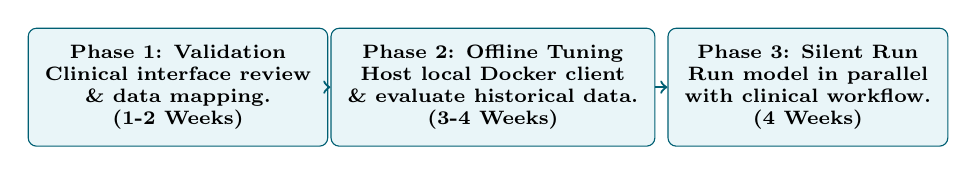
\begin{tikzpicture}[node distance=2.2cm, every node/.style={fill=white, draw=clinicTeal, rounded corners=3pt, font=\scriptsize\bfseries, inner sep=6pt, align=center}]
        
        \node (p1) [fill=lightTeal] {\textbf{Phase 1: Validation} \\ Clinical interface review \\ \& data mapping. \\ (1-2 Weeks)};
        
        \node (p2) [right of=p1, xshift=1.8cm, fill=lightTeal] {\textbf{Phase 2: Offline Tuning} \\ Host local Docker client \\ \& evaluate historical data. \\ (3-4 Weeks)};
        
        \node (p3) [right of=p2, xshift=1.8cm, fill=lightTeal] {\textbf{Phase 3: Silent Run} \\ Run model in parallel \\ with clinical workflow. \\ (4 Weeks)};
        
        \draw[->, thick, clinicTeal] (p1) -- (p2);
        \draw[->, thick, clinicTeal] (p2) -- (p3);
    \end{tikzpicture}
    
    \vspace{0.4cm}
    \begin{block}{Goal of the Pilot Program}
        \scriptsize
        Evaluate the early-warning accuracy of FPDAF in parallel with daily clinical operations, with zero risk to patients, in order to prove diagnostic utility and safety.
    \end{block}
\end{frame}


% --- SLIDE 8: JOIN THE PILOT ---
\begin{frame}
    \centering
    \vspace{1cm}
    {\Huge \textbf{\textcolor{clinicTeal}{Join the Clinical Pilot Program}}} \\
    \vspace{0.4cm}
    {\large Partner with us to build explainable, secure, and privacy-preserving healthcare AI.} \\
    \vspace{0.8cm}
    
    \begin{block}{Primary Contacts}
        \centering
        \scriptsize
        CB.SC.U4CSE23547 | SHEELA AKSHAR SAKHI (Team Lead) | aksharsakhi@gmail.com \\
        \vspace{0.1cm}
        Project Guides: Dr. G R Ramya \& Dr. Vandhana S \\
        Amrita School of Computing, Coimbatore Campus
    \end{block}
    
    \vspace{0.4cm}
    {\large Questions? Let's Collaborate.}
\end{frame}

\end{document}
